\documentclass[tikz,border=10pt]{standalone}
\usepackage{tikz}
\usetikzlibrary{arrows.meta,positioning}

\begin{document}
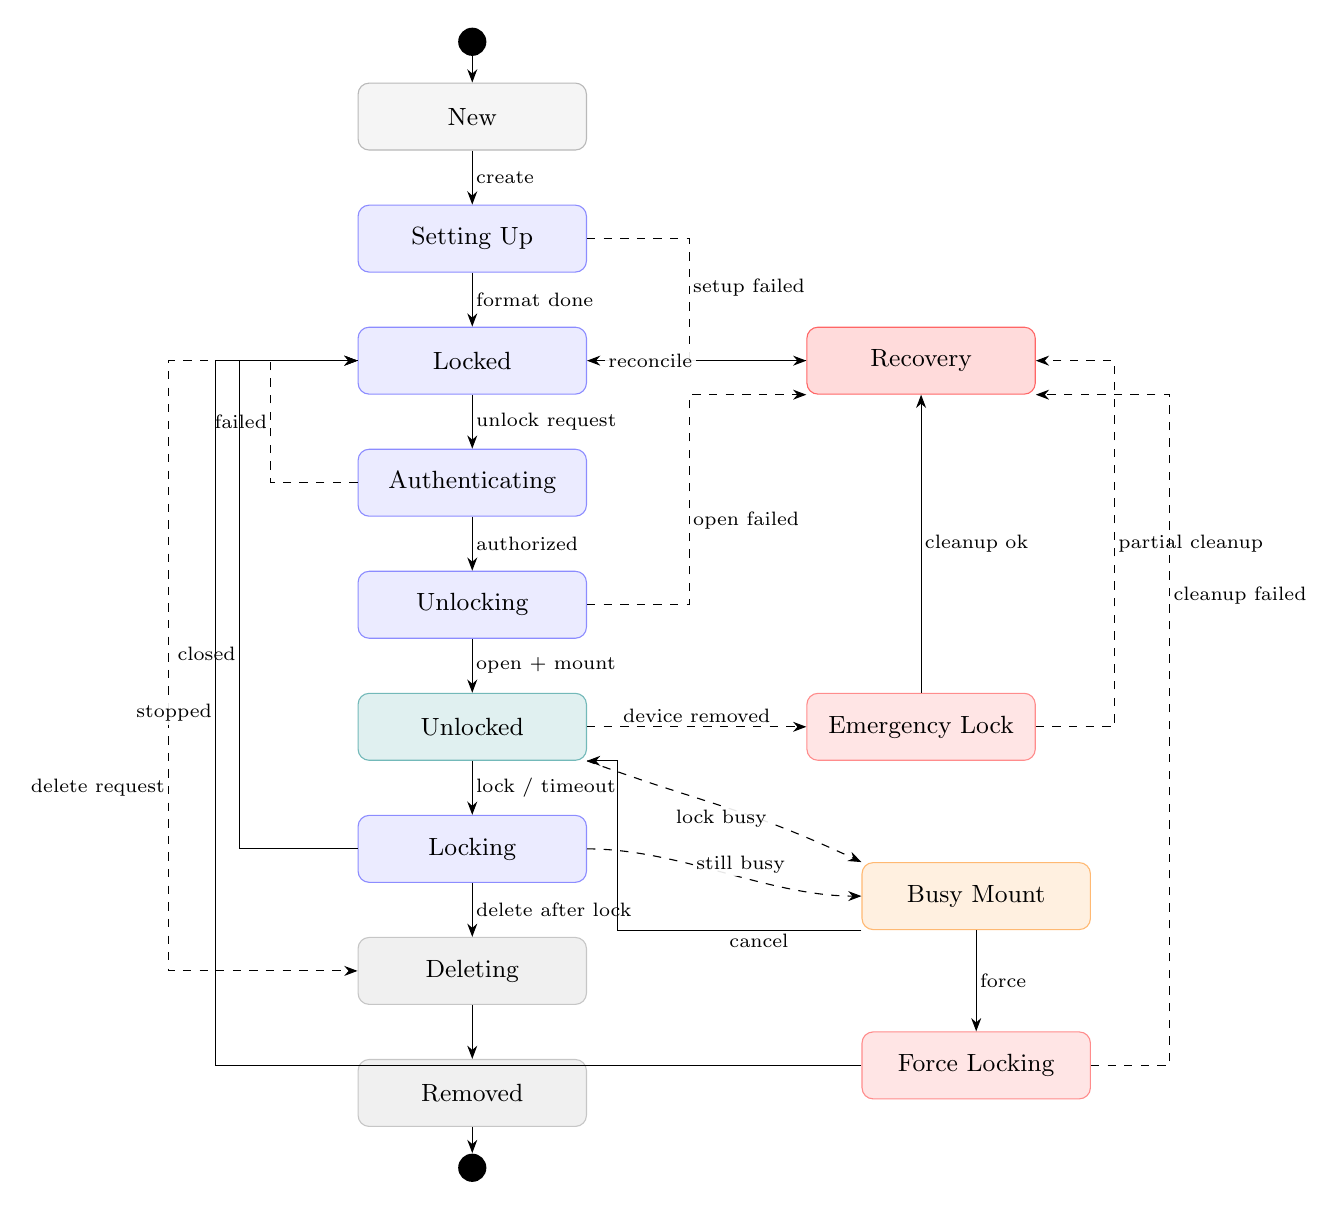
\begin{tikzpicture}[
  >=Stealth,
  box/.style={
    draw,
    rounded corners=4pt,
    minimum width=2.9cm,
    minimum height=0.85cm,
    align=center,
    font=\small,
    fill=gray!8,
    draw=gray!55
  },
  main/.style={box, fill=blue!8, draw=blue!45},
  active/.style={box, fill=teal!12, draw=teal!55},
  warn/.style={box, fill=orange!12, draw=orange!55},
  danger/.style={box, fill=red!10, draw=red!45},
  recover/.style={box, fill=red!14, draw=red!60},
  gone/.style={box, fill=gray!12, draw=gray!45},
  flow/.style={->, thin},
  alt/.style={->, dashed, thin},
  label/.style={font=\scriptsize, fill=white, inner sep=1.2pt, text opacity=1, fill opacity=0.9}
]

% Main lifecycle column
\node[box]    (new)       at (0, 0)      {New};
\node[main]   (setup)     at (0,-1.55)   {Setting Up};
\node[main]   (locked)    at (0,-3.10)   {Locked};
\node[main]   (auth)      at (0,-4.65)   {Authenticating};
\node[main]   (unlocking) at (0,-6.20)   {Unlocking};
\node[active] (unlocked)  at (0,-7.75)   {Unlocked};
\node[main]   (locking)   at (0,-9.30)   {Locking};
\node[gone]   (deleting)  at (0,-10.85)  {Deleting};
\node[gone]   (removed)   at (0,-12.40)  {Removed};

% Exceptional and recovery paths
\node[recover] (recovery)  at (5.7,-3.10)  {Recovery};
\node[danger]  (emergency) at (5.7,-7.75)  {Emergency Lock};
\node[warn]    (busy)      at (6.4,-9.90)  {Busy Mount};
\node[danger]  (force)     at (6.4,-12.05) {Force Locking};

% Start and end markers
\node[circle, fill=black, inner sep=3.6pt] (start) at (0, 0.95) {};
\node[circle, fill=black, inner sep=3.6pt, double, double distance=2pt] (end) at (0,-13.35) {};

% Normal lifecycle
\draw[flow] (start) -- (new);
\draw[flow] (new) -- node[label,right]{create} (setup);
\draw[flow] (setup) -- node[label,right]{format done} (locked);
\draw[flow] (locked) -- node[label,right]{unlock request} (auth);
\draw[flow] (auth) -- node[label,right]{authorized} (unlocking);
\draw[flow] (unlocking) -- node[label,right]{open + mount} (unlocked);
\draw[flow] (unlocked) -- node[label,right]{lock / timeout} (locking);
\draw[flow] (deleting) -- (removed);
\draw[flow] (removed) -- (end);

% Common alternative outcomes
\draw[alt] (auth.west) -- ++(-1.1,0) |- node[label,left,pos=0.25]{failed} (locked.west);
\draw[flow] (locking.west) -- ++(-1.5,0) |- node[label,left,pos=0.20]{closed} (locked.west);
\draw[alt] (locked.west) -- ++(-2.4,0) |- node[label,left,pos=0.35]{delete request} (deleting.west);
\draw[flow] (locking) -- node[label,right]{delete after lock} (deleting);

% Emergency, busy mount, and force-lock paths
\draw[alt] (unlocked.east) -- node[label,above]{device removed} (emergency.west);
\draw[alt] (unlocked.south east) to[out=-20,in=155,looseness=1.15]
  node[label,below,pos=0.48]{lock busy} (busy.north west);
\draw[alt] (locking.east) to[out=0,in=180,looseness=0.85]
  node[label,above,pos=0.56]{still busy} (busy.west);
\draw[flow] (busy.south west) -- node[label,below,pos=0.42]{cancel} ++(-3.1,0) |- (unlocked.south east);
\draw[flow] (busy) -- node[label,right]{force} (force);
\draw[flow] (force.west) -- ++(-8.2,0) |- node[label,left,pos=0.25]{stopped} (locked.west);

% Recovery paths
\draw[flow] (emergency) -- node[label,right]{cleanup ok} (recovery);
\draw[alt] (emergency.east) -- ++(1.0,0) |- node[label,right,pos=0.25]{partial cleanup} (recovery.east);
\draw[alt] (setup.east) -- ++(1.3,0) |- node[label,right,pos=0.20]{setup failed} (recovery.west);
\draw[alt] (unlocking.east) -- ++(1.3,0) |- node[label,right,pos=0.20]{open failed} (recovery.south west);
\draw[alt] (force.east) -- ++(1.0,0) |- node[label,right,pos=0.35]{cleanup failed} (recovery.south east);
\draw[flow] (recovery.west) -- ++(-1.4,0) |- node[label,left,pos=0.25]{reconcile} (locked.east);

\end{tikzpicture}
\end{document}
